\documentclass[11pt]{article}

% Problem Set Template

% Based on Paolo Adajar's template: https://github.com/padajar/paolo-pset/tree/main

% NOTE: Add in the relevant information to the commands below; or, if you'll be using the same information frequently, add these commands at the top of paolo-pset.tex file. 
\newcommand{\assignment}{Problem Set 1}
\newcommand{\duedate}{2024-09-01}

% NOTE: Defining collaborators is optional; to not list collaborators, comment out the line below.
% \newcommand{\collaborators}{Alyssa P. Hacker (\texttt{aphacker}), Ben Bitdiddle (\texttt{bitdiddle})}

\input{../ps_tex_template.tex}

% NOTE: To compile a version of this pset without problems, solutions, or reflections, uncomment the relevant line below.

%\excludeversion{problem}
%\excludeversion{solution}
%\excludeversion{reflection}

\begin{document}	
	
% Use the \psetheader command at the beginning of a pset. 
\psetheader
	
\begin{enumerate}
    \item \begin{problem} 
        What is $2+2$? 
    \end{problem}
    
    4

    \item \begin{problem}
        [MWG 1.1] What is the airspeed velocity of an unladen swallow?
    \end{problem}
    
    An African or European swallow?

    \item \begin{problem}
        Do some math
    \end{problem}
    
    $$
    3 + 3 = 6
    $$

    \item \begin{problem}
        Include a figure
    \end{problem}

    \begin{center}
        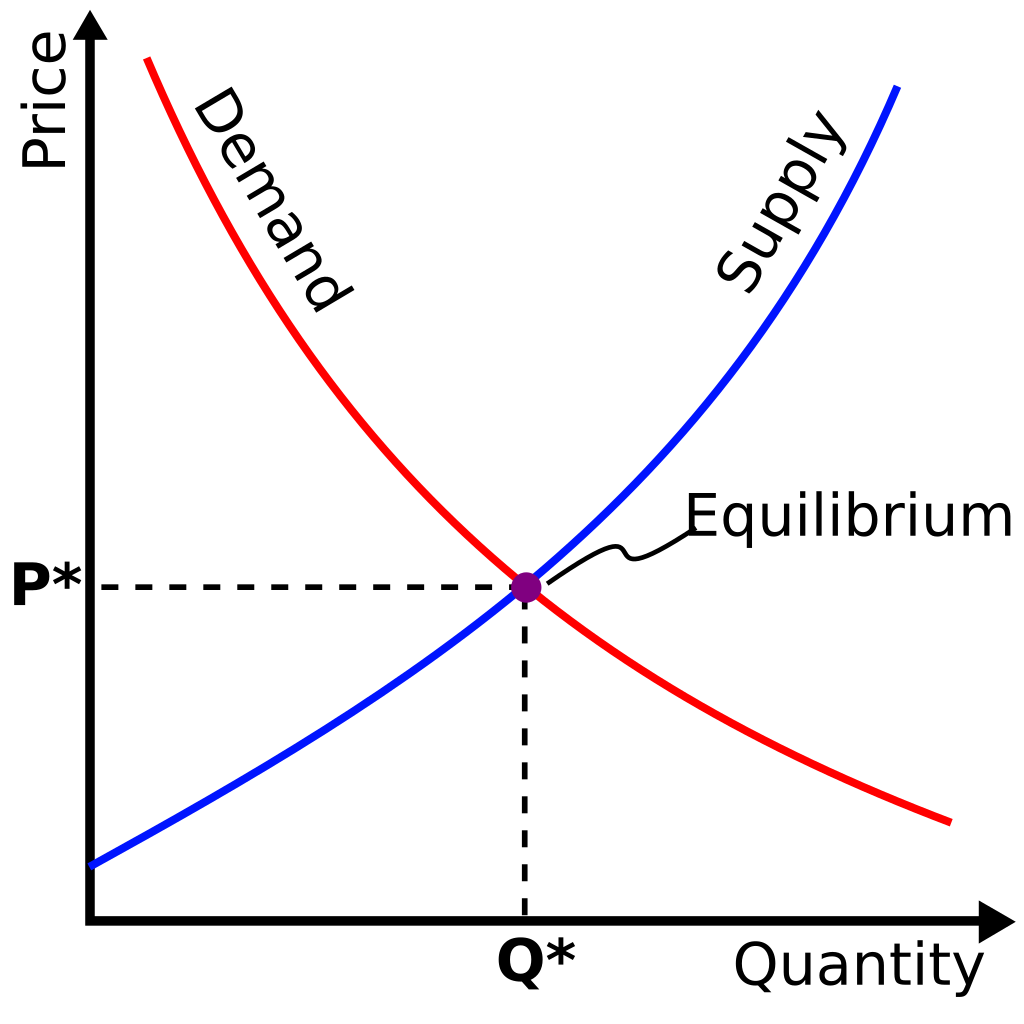
\includegraphics[width=0.25\textwidth]{../figures/supply_demand.png}
    \end{center}
    
\end{enumerate}

	
\end{document}